The motion planner was tested using the compass-gait robot over terrains with small step changes in height. The lack of knees in the robot made it challenging for the robot to reliably complete motions over even small step ups in the terrain. This is not an issue for more complex robots, but since these are also significantly more difficult to model, validation of this work on robots with knees is deferred to later work.

Another limitation of the efficacy of the testing on the compass gait robot is that the ground avoidance measures in the motion planning algorithm must be disabled, since it is not possible for the two link walker to avoid scuffing its leg on the ground. This is not considered to be a serious concern, since kinematic feasibility testing is a fairly trivial process and the extent to which the robot intersects with the terrain is limited by virtue of planning the foot placement.

\subsection{Behaviour of planner}
\begin{figure}
\centering
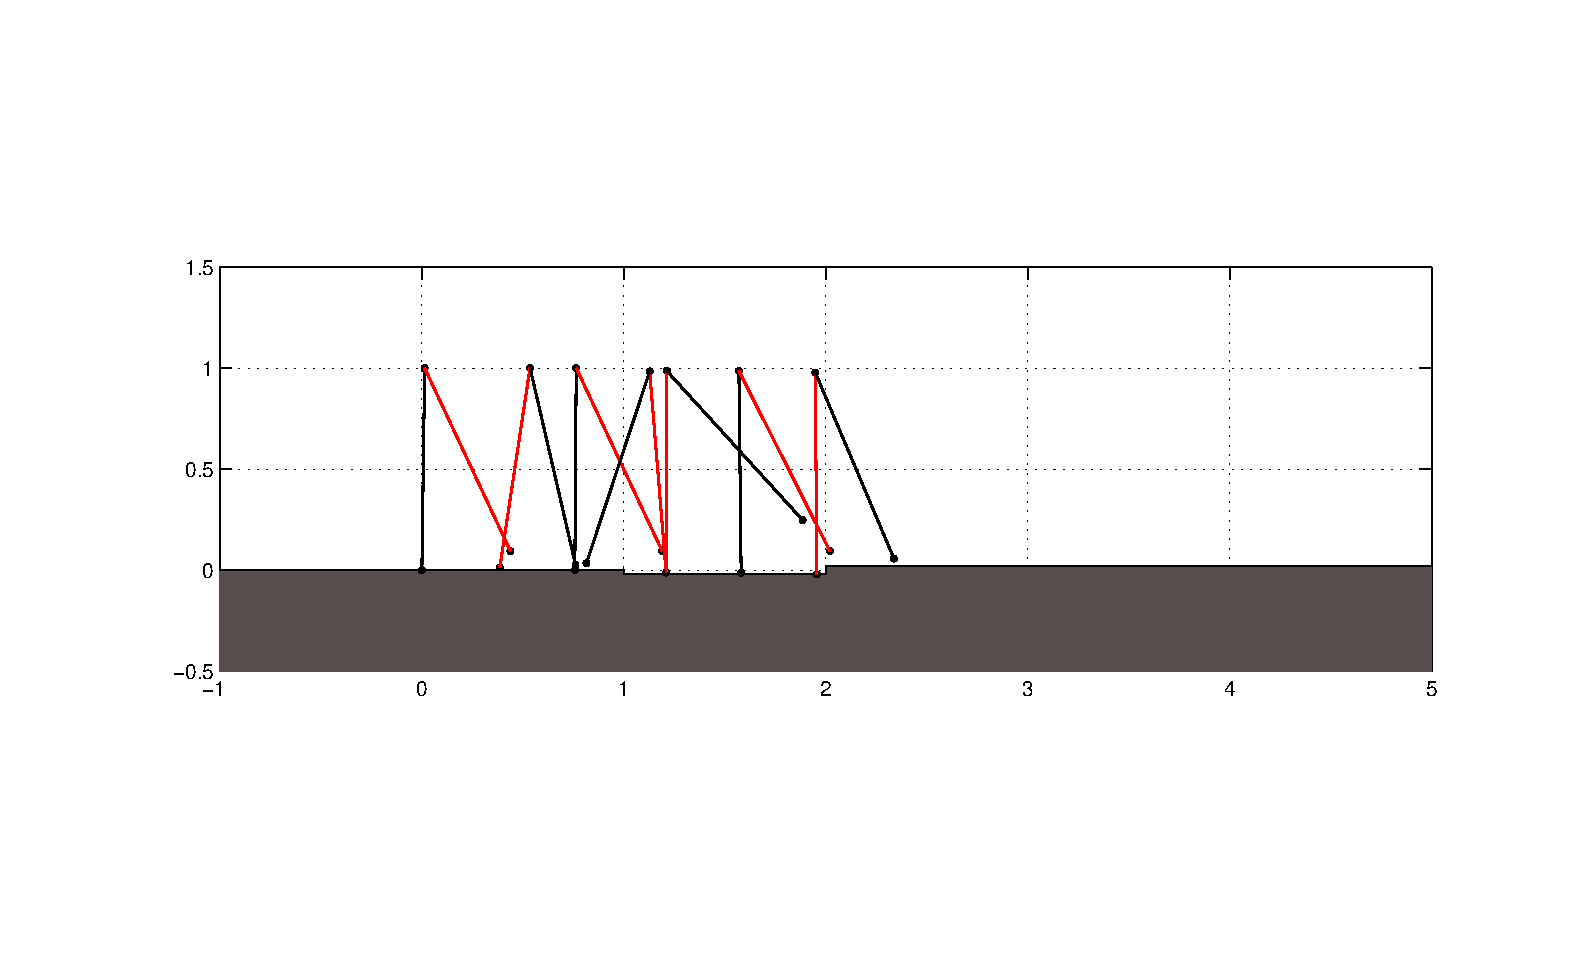
\includegraphics[width=\linewidth]{7Results/stepupfault}
\caption{Example trajectory of the two link robot unable to complete a modest step-up}
\label{fig:stepupfault}
\end{figure}

It was found that the motion planner was prone to failure where it attempted to add kinetic energy in order to be able to step up over even modest jumps in the terrain. This matches the results in Section \ref{sec:reskineng}; the motion planner expects a given primitive to add a certain amount of energy, but the post-impact loss of velocity is greater than anticipated. As shown in Figure \ref{fig:stepupfault}, this causes the planner to fail after the robot impacts with the higher terrain; up to the step-up, the robot is adding kinetic energy, seen in the fact that it swings its leg forward. However, after impact, it is found that there is less energy than anticipated, and the planner fails to find a feasible sequence of footsteps.

Otherwise than in this matter, the results obtained from the motion planner were favourable. In Figure \ref{fig:slowdown}, we observe that the walker places the front foot ahead of itself less as it traverses down a slope to keep the velocity from exceeding that required for the assumption of a constant coefficient of static friction to be valid.

\begin{figure}
\centering
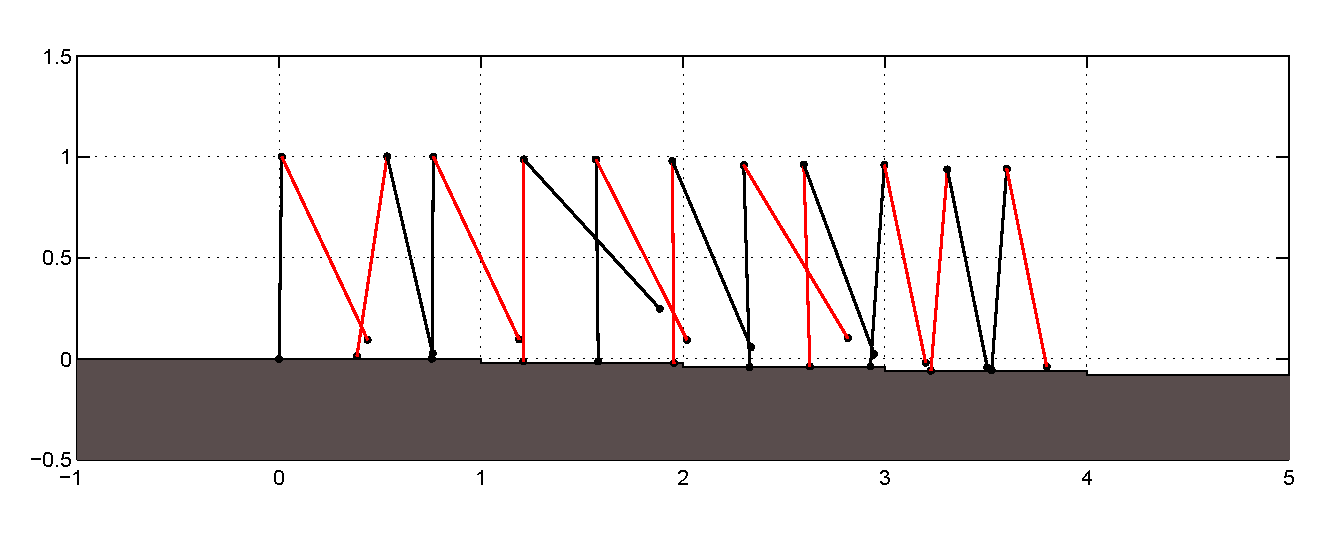
\includegraphics[width=\linewidth]{7Results/slowdown}
\caption{Trajectory of the robot walking down a stepped incline}
\label{fig:slowdown}
\end{figure}

\subsection{Running time}
Using the library mentioned in the previous section which contains 33 275 virtual constraints, the average and maximum running time of the planner over a set trajectory was measured using differing values of the look ahead, $k$. This produced the graph in Figure \ref{fig:lookahead}. Note that the running time is linear in $k$, corresponding much more closely with the best-case running time than the worst-case, as presented in Section \ref{sec:complexity}.

\begin{figure}
\centering
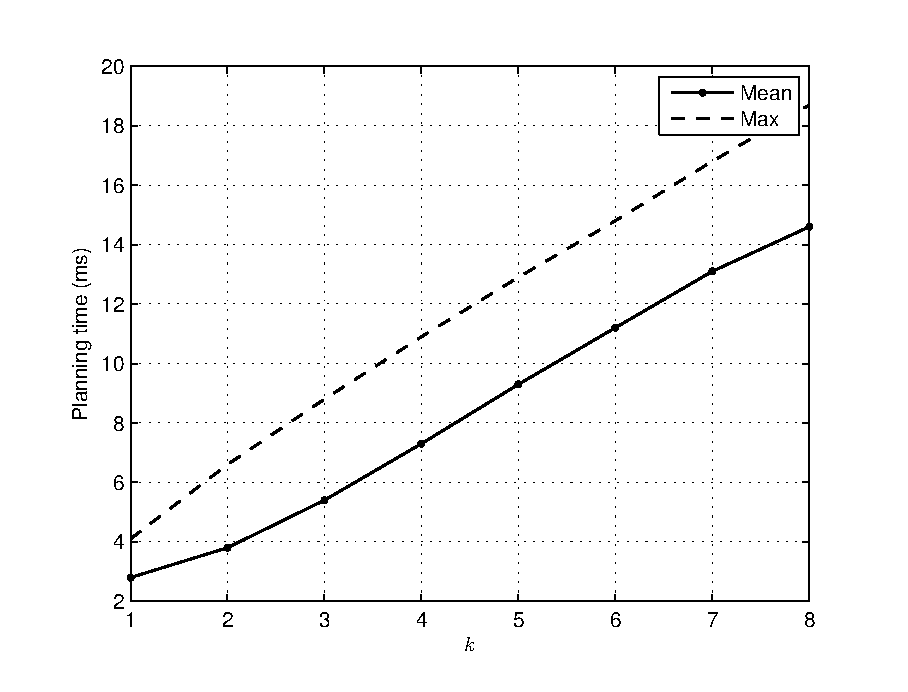
\includegraphics[width=0.6\linewidth]{7Results/lookahead}
\caption{Growth in running time with varying look-ahead distance $k$}
\label{fig:lookahead}
\end{figure}

The running time of the algorithm for more complicated robots in principle need not increase, since the algorithm itself deals only with the phase variable, which is one dimensional regardless of the complexity of the robot. However, it should be noted that a robot with more degrees of freedom likely requires more motion primitives to span the range of available motions. Even so, with the logarithmic increase in the dimensions of the library, the running time should be expected to be very fast.

It is notable that there are numerous improvements that can be made to the running time; in \cite{manchester13planning}, the number of traversals down the decision tree was significantly reduced through utilising an energy-based heuristic, as described in Section \ref{sec:heuristic}. In addition, the implementation of the code in MATLAB is not expected to be as efficient as an implementation in C, for example. These results should imply that running this motion planning algorithm on a microcontroller is not infeasible.

\subsection{Optimality of chosen VCs} \label{sec:resnom}
The motion planning algorithm does not make any explicit attempt to choose an optimal sequence of motion primitives. Rather, the virtual constraints are chosen on the basis of a loose notion that minimising the velocity of the virtual constraint at the critical point (subject to it being greater than zero) should produce a reasonable sequence of constraints. The choice of virtual constraints on the basis of energy heuristics is not considered here.

Recall from Section \ref{sec:optmethod} that the virtual constraints are optimised for a particular initial velocity. For other velocities, there is no guarantee of torque minimisation. An instructive inquiry, therefore, is to inspect the velocities of the chosen virtual constraints for proximity to the nominal velocity. Table \ref{tab:nomvel} presents the average deviation from the nominal velocity of virtual constraints over different terrain profiles. All of these results were produced with an initial velocity of $\dot{\theta}_0^2=7.1~\mathrm{rad}^2/s^2$.

\begin{table}
	\centering
	\begin{tabular}{c | c | c | c }
		Terrain profile & Mean & Standard deviation & Median \\ \hline
		Flat ground & -6.30 \% & 6.37 \% & -4.27 \% \\
		Step up terrain & -8.88 \% & 6.94 \% & -8.88 \% \\
		Step down terrain & -6.49 \% & 4.35 \% & -5.10 \%\\
	\end{tabular}
	\caption{Deviation of observed $\dot{\theta}^2$ from $\dot{\theta}^{*^2}$ in simulated trajectories}
	\label{tab:nomvel}
\end{table}

We observe a very definite and sustained trend of the initial velocity being at a small but significant offset from the nominal velocity, with all three terrain types producing similar data. The results presented here can be used to inform the design of the motion primitive library. Indeed, if the optimality of the library in real-time is a significant concern, an iterative approach to choosing the nominal velocity should be used. The definition of the nominal velocities as presented in \ref{sec:optmethod} are a good first guess based upon having no data from simulations of the motion planner. Setting up the initial conditions of the simulation is an important factor in the production of these results. There is unavoidable; in its current form, the planning problem requires an initial velocity in order to work.